\section{Vehicle Build and Manufacture}
\label{sec:vehicleBuildAndManufacture}
  The project focus was primarily the design of the rover model and the accompanying software and electronic systems. However, a large portion of the effort was put into the manufacture of the model which will be covered briefly in this section. The manufacture process began with plans and analysis of the design, collation of a bill of materials and finally manufacture and assembly of the rover.
  
  \subsection{Manufacturing Plan}
    \subsubsection{Analysis of 3D Components}
      Many of the 3D components formed part of the suspension system, the mechanism which took on the largest stresses compared to the rest of the model. For this reason, correct printing orientations were important for the strength and robustness of the rover. While the printing direction (layer direction) and the coupling of it with both geometrical limitations and stress orientations were taken into account during the design of each piece, a further visual analysis was performed on each part to decide upon the most suitable printing orientation.
      
    \subsubsection{Design Preparation}
      At this point, the entire design was in the form of 3D models and 2D CAD drawings. Printing of the 3D components required exporting of the design files to the correct format. Manufacturer specifications required the object data in \mintinline{js}{STL} format, an export operation provided by the 3D CAD tool used to design the components. Each file was exported and verified.
      
      The laser cutting process for the acrylic body panels required the 2D detail drawings to be in \mintinline{js}{PDF} format which was performed and verified as well.
    
  \subsection{Bill of Materials}
    Table~\ref{tab:BOM} shows the bill of materials for the mechanical and electrical systems of the rover.
  
    \begin{table}[H]
    \centering
    \begin{tabular}{@{}lll@{}}
    \toprule
    Item                               & Description                                     & Quantity      \\ \midrule
    Intel Edison                       & With Arduino Extension Board                    & 1             \\
    Adafruit PWM Shield                & 16 Channel, I$^2$C                              & 1             \\
    XL4015 Buck DC-DC Converter        & 5A, 1.25-36V Output                             & 1             \\
    HC-SR04 Ultrasonic Distance Sensor &                                                 & 3             \\
    Hextronik HXT900 9G Servo          & Plastic gear                                    & 10            \\
    Servo Extension Cables             & 150mm                                           & 10            \\
    USB Web Camera                     & msi Starcam Flip - UVC compatible               & 1             \\
    Lithium Polymer Battery Pack       & 3 Cell, 100mAh                                  & 1             \\
    LM358 Operational Amplifier        & DIP                                             & 3             \\
    10$\mu$F Capacitor                 &                                                 & 3             \\
    Dual Row Male Headers              & 4-pins wide                                     & 3             \\
    Single Row Male Headers            & 4-pins wide                                     & 3             \\
    Single Row Female Headers          & 4-pins wide                                     & 12            \\
    M2 Hex Nut                         &                                                 & 58            \\
    M2 Pan Slotted Screw               &                                                 & 58            \\
    M2 Narrow Washer                   &                                                 & $\approx$ 100 \\
    M3 Hex Nut                         &                                                 & 80            \\
    M3 Pan Slotted Screw               &                                                 & 74            \\
    M3 Narrow Washer                   &                                                 & $\approx$ 50  \\
    Round Extrude Aluminium Tube       & 15.88mm$\times$1.62mm                           & 1m            \\
    Solid Aluminium Rod                & 6mm                                             & 1m            \\
    Ball Bearings                      & 5$\times$16$\times$5, Stainless steel, shielded & 13            \\
    Neodymium Disc Magnets             & 3mm$\times$2mm                                  & 8             \\
    Acrylic Sheet                      & 3mm, Soft white, A3                             & 1             \\
    3D Printed Components              & As exported from CAD                            &               \\ \bottomrule
    \end{tabular}
    \caption{Table of the bill of materials for the mechanical and electrical systems of the rover.}
    \label{tab:BOM}
    \end{table}
  
  \subsection{Vehicle Assembly}
    \subsubsection{Manufacture of 3D Parts}
      After the analysis on the designed 3D components was performed and the files exported to the correct format, one of many materials that could be used as filament in the printing process was chosen. The two most common of these materials were PLA (Polylactic Acid) and ABS (Acrylonitrile Butadiene Styrene), each a type of thermoplastic with associated thermal and physical properties. The more widely used of the two was PLA due to a significantly lower glass-point temperature meaning the required temperature of the heating element of the printer nozzle be less than that when printing in ABS. However, it was found that PLA was more brittle, allowing for less flexure before cracking and shattering. ABS, the same plastic used for Lego bricks, allowed for greater flexibility and was observed to plastically deform long before cracking. For this reason, ABS was chosen as it would offer the durability in the pieces that were to undergo higher bending stresses (such as the joints of the suspension system).
      
      Due to the volume of printing required, external, local ABS printing services had to be found to have the parts manufactured. Multiple companies were contacted for quotes, however, the budget of the project was not able to include the cost of such a service. A company was found, ProtoLink 3D\footnote{ProtoLink 3D - \url{http://www.protolink3d.co.za/}}, which was willing to fully sponsor the project.
      
      Once the parts were printed, all support material and extra plastic was removed and prepared for assembly. All the holes were inspected for correct position for alignment with other pieces and for size. Features that were not correct were altered either using a drill press or a hot piece of steel. Figure~\ref{fig:mechBuild-removalOfPlasticSupport} shows the removal of support material from a component.
      
      \begin{figure}[h!]
        \centering
        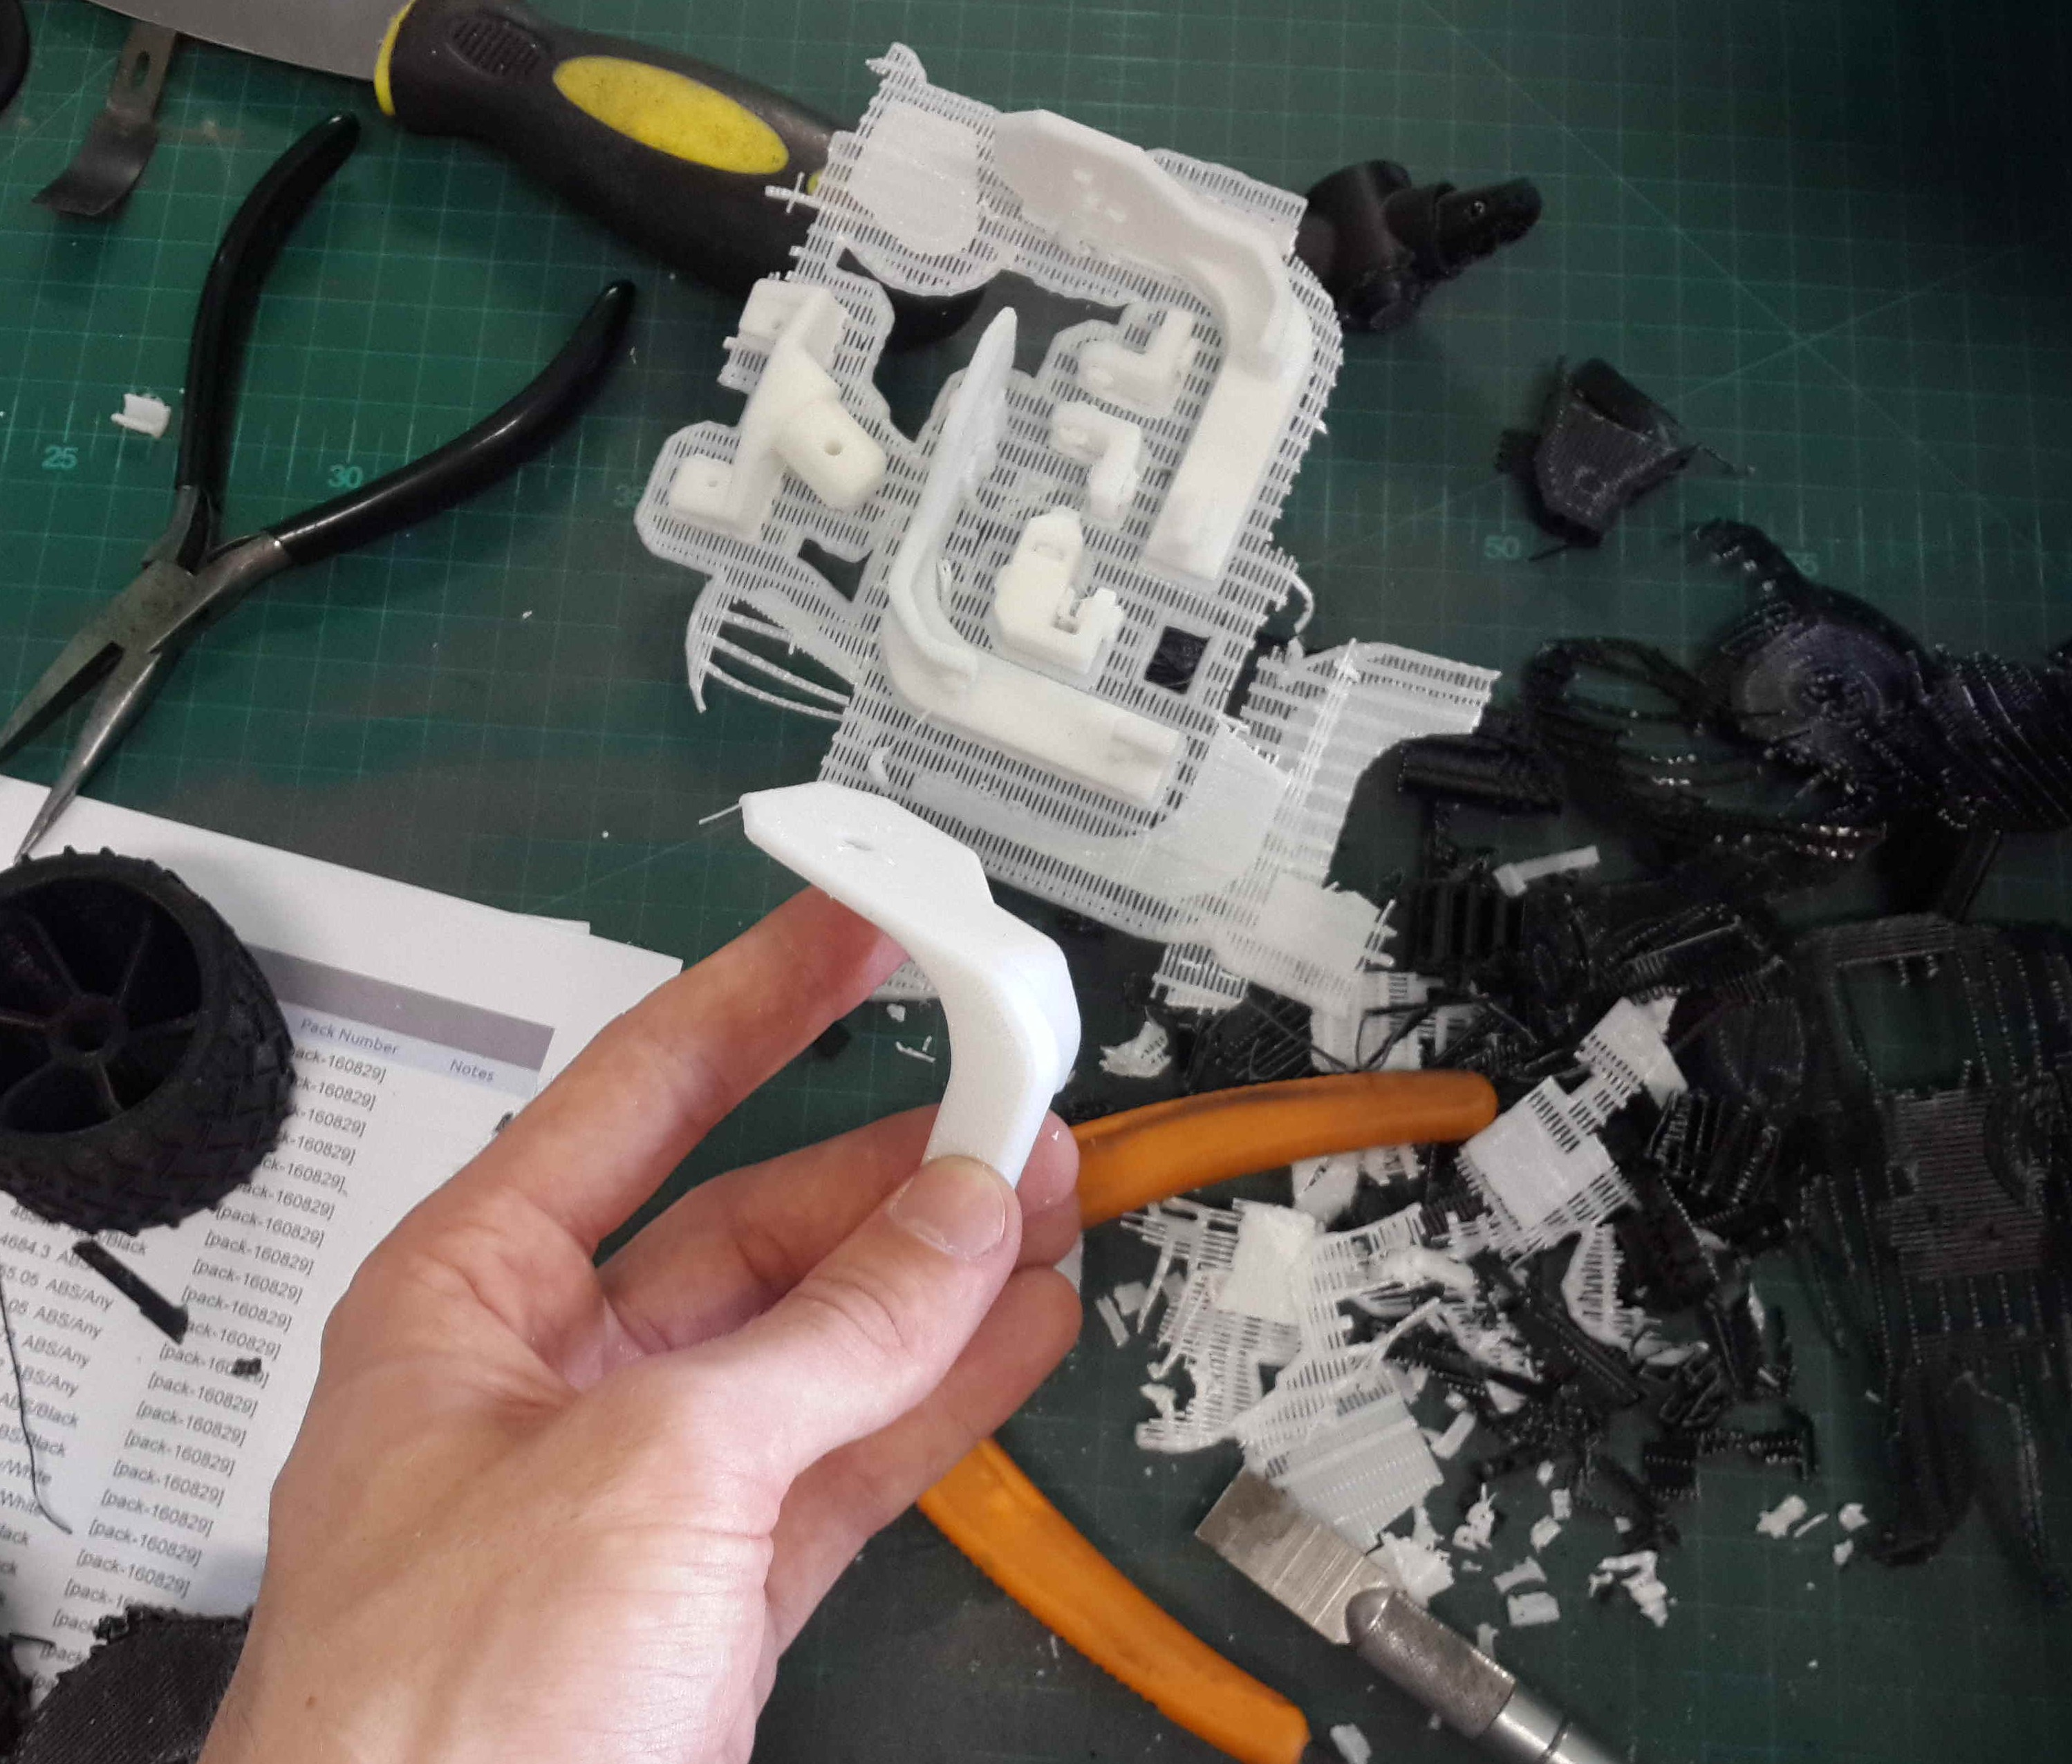
\includegraphics[width=0.6\linewidth]{figures/mechBuild-removalOfPlasticSupport}
        \caption[Image of a printed component (a wheel strut) with the plastic support and extra material removed.]{Image of a printed component (a wheel pivot) with the plastic support and extra material removed.}
        \label{fig:mechBuild-removalOfPlasticSupport}
      \end{figure}
    
    \subsubsection{Assembly of Suspension and Body}
      The five acrylic panels that made up the body component of the rover were joined and glued using Tensol Number 17. This resulted in the tabbed edges of the panels to fuse together providing a strong structure for external and internal mounting of components. 
      
      Assembly of the suspension system involved the printed joints, aluminium tube pieces, aluminium shafts and bearings. The aluminium tubing was cut to size and the edges finished. Holes were drilled at each end of the tube pieces for fastening to the printed joint components. Aluminium shafts required for the rocker and bogies joints as well as the center wheels were also cut to size and chamfered. The bearings were press-fit into the printed joints and the shafts were inserted into the mounted bearings using a stationary drill press. Some of the shafts were too thick to be easily but securely pressed into the bearings and had to be reduced in size. The aluminium tube pieces were press-fit onto the hexagonal joint plugs and secured using nuts and bolts. Figure~\ref{fig:mechBuild-completedSuspensionSide} shows one side of the suspension system without the servo-mounted components.
      
      The servos and servo horns were also fastened to the wheel pivots, struts and the wheels themselves, completing the assembly of the body and suspension system.
      
      \begin{figure}[h!]
        \centering
        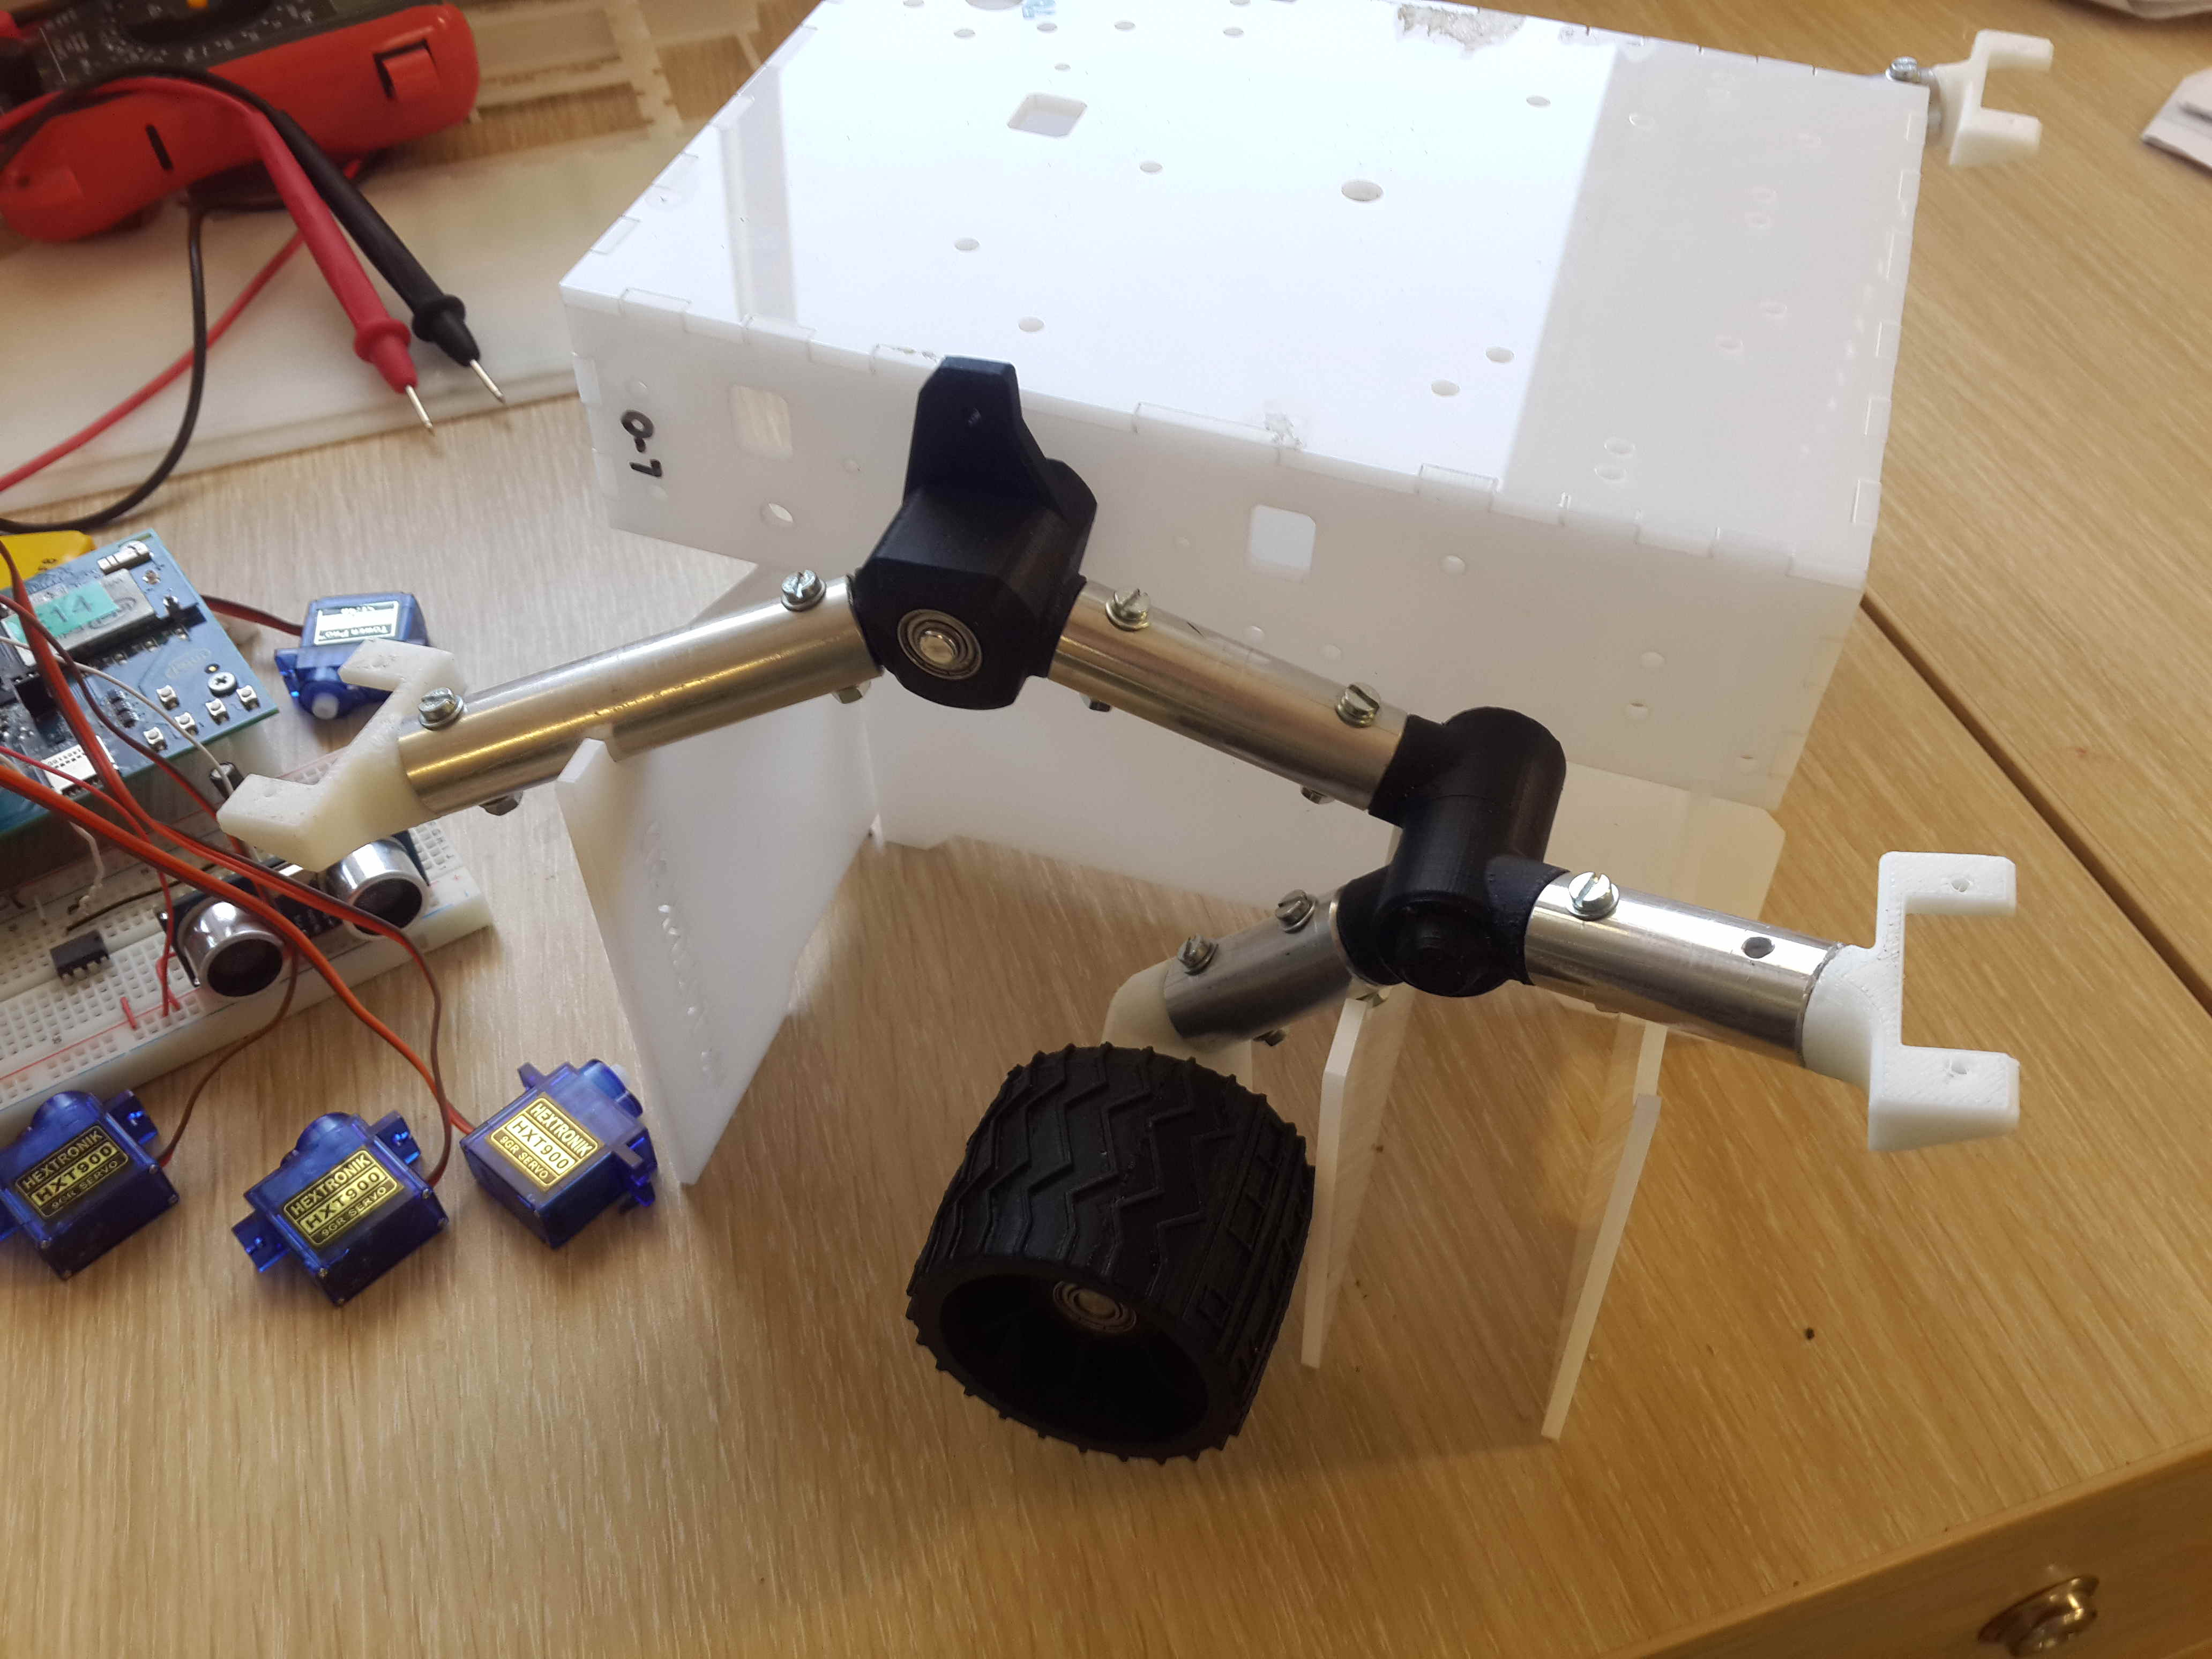
\includegraphics[width=0.6\linewidth]{figures/mechBuild-completedSuspensionSide}
        \caption[Image of one completed side of the suspension system before servo-related components were assembled.]{Image of one completed side of the suspension system before servo-related components were assembled.}
        \label{fig:mechBuild-completedSuspensionSide}
      \end{figure}
      
    \subsubsection{Internal Electronics Mounting}
      As designed, the internal compartment of the body component of the rover was to be used for mounting of the electronic system. The design of the top panel of the body included holes aligned with mounting points on the Intel Edison board and these were used to fasten the board to the underside of the top panel. Below that, the Adafruit PWM extension module was fitted to the Intel Edison board and the length of the Intel Edison board mounts adjusted so that the rocker joint shaft, which passed through the width of the rover body, fitted between the board and the PWM extension module. The length adjustment also took into account the height of the servo cables plugged into the PWM module and the interference of those with the bottom cover of the body.
      
      An acrylic mounting component, cut from the same acrylic sheet used for the body panels, was fastened to the PWM module to provide a mounting platform for the custom pulse to analog converter boards and the buck DC to DC converter module. the acrylic mounting component also provided insulation of the high power portion of the system from the Intel Edison board and PWM module.
      
      Figure~\ref{fig:mechBuild-internalElectronicsMountingPlan} shows the mounting and wiring plan used during the assembly of the rover and Figure~\ref{fig:mechBuild-internalElectronics} shows the completed electronics system as mounted.
      
      \begin{figure}[h!]
        \centering
        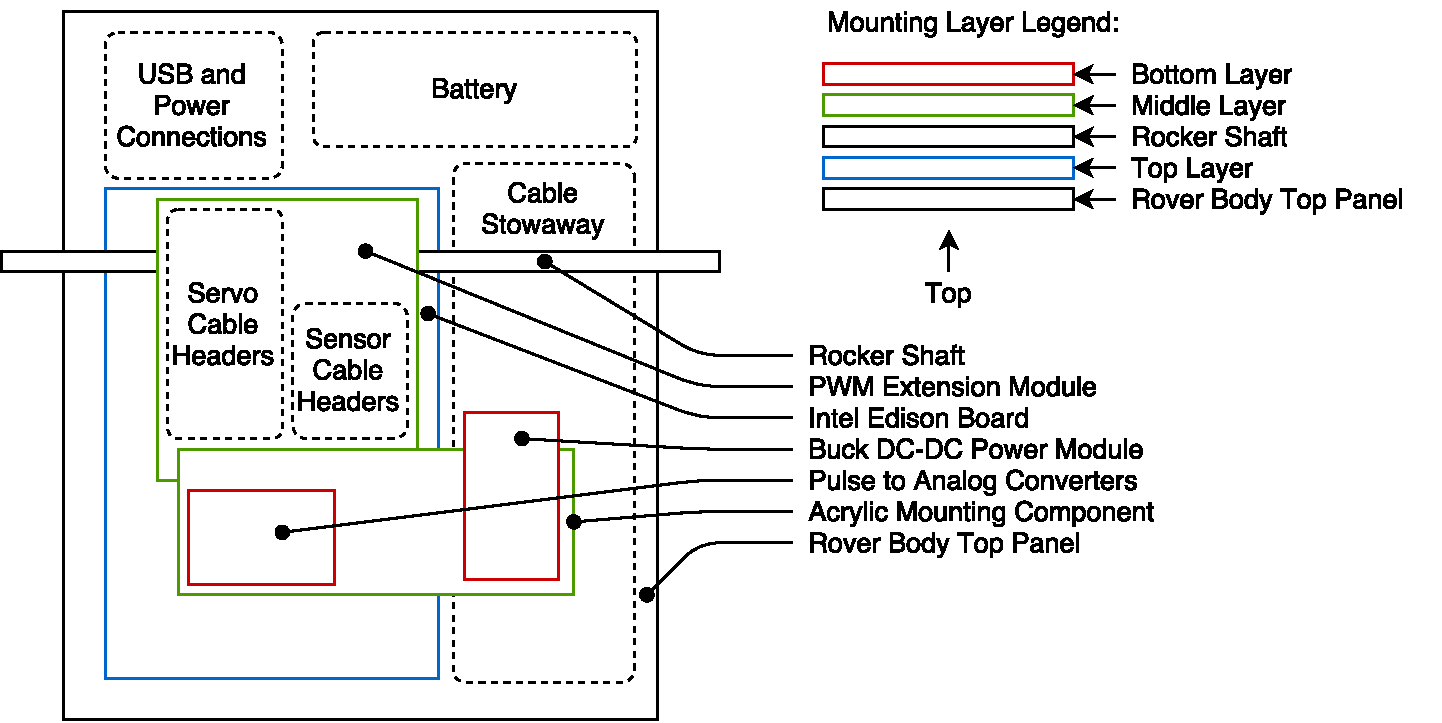
\includegraphics[width=0.9\linewidth]{figures/mechBuild-internalElectronicsMountingPlan}
        \caption[Diagram of the rover body internal electronics mounting plan as seen from below.]{Diagram of the rover body internal electronics mounting plan as seen from below.}
        \label{fig:mechBuild-internalElectronicsMountingPlan}
      \end{figure}
      
      \begin{figure}[h!]
        \centering
        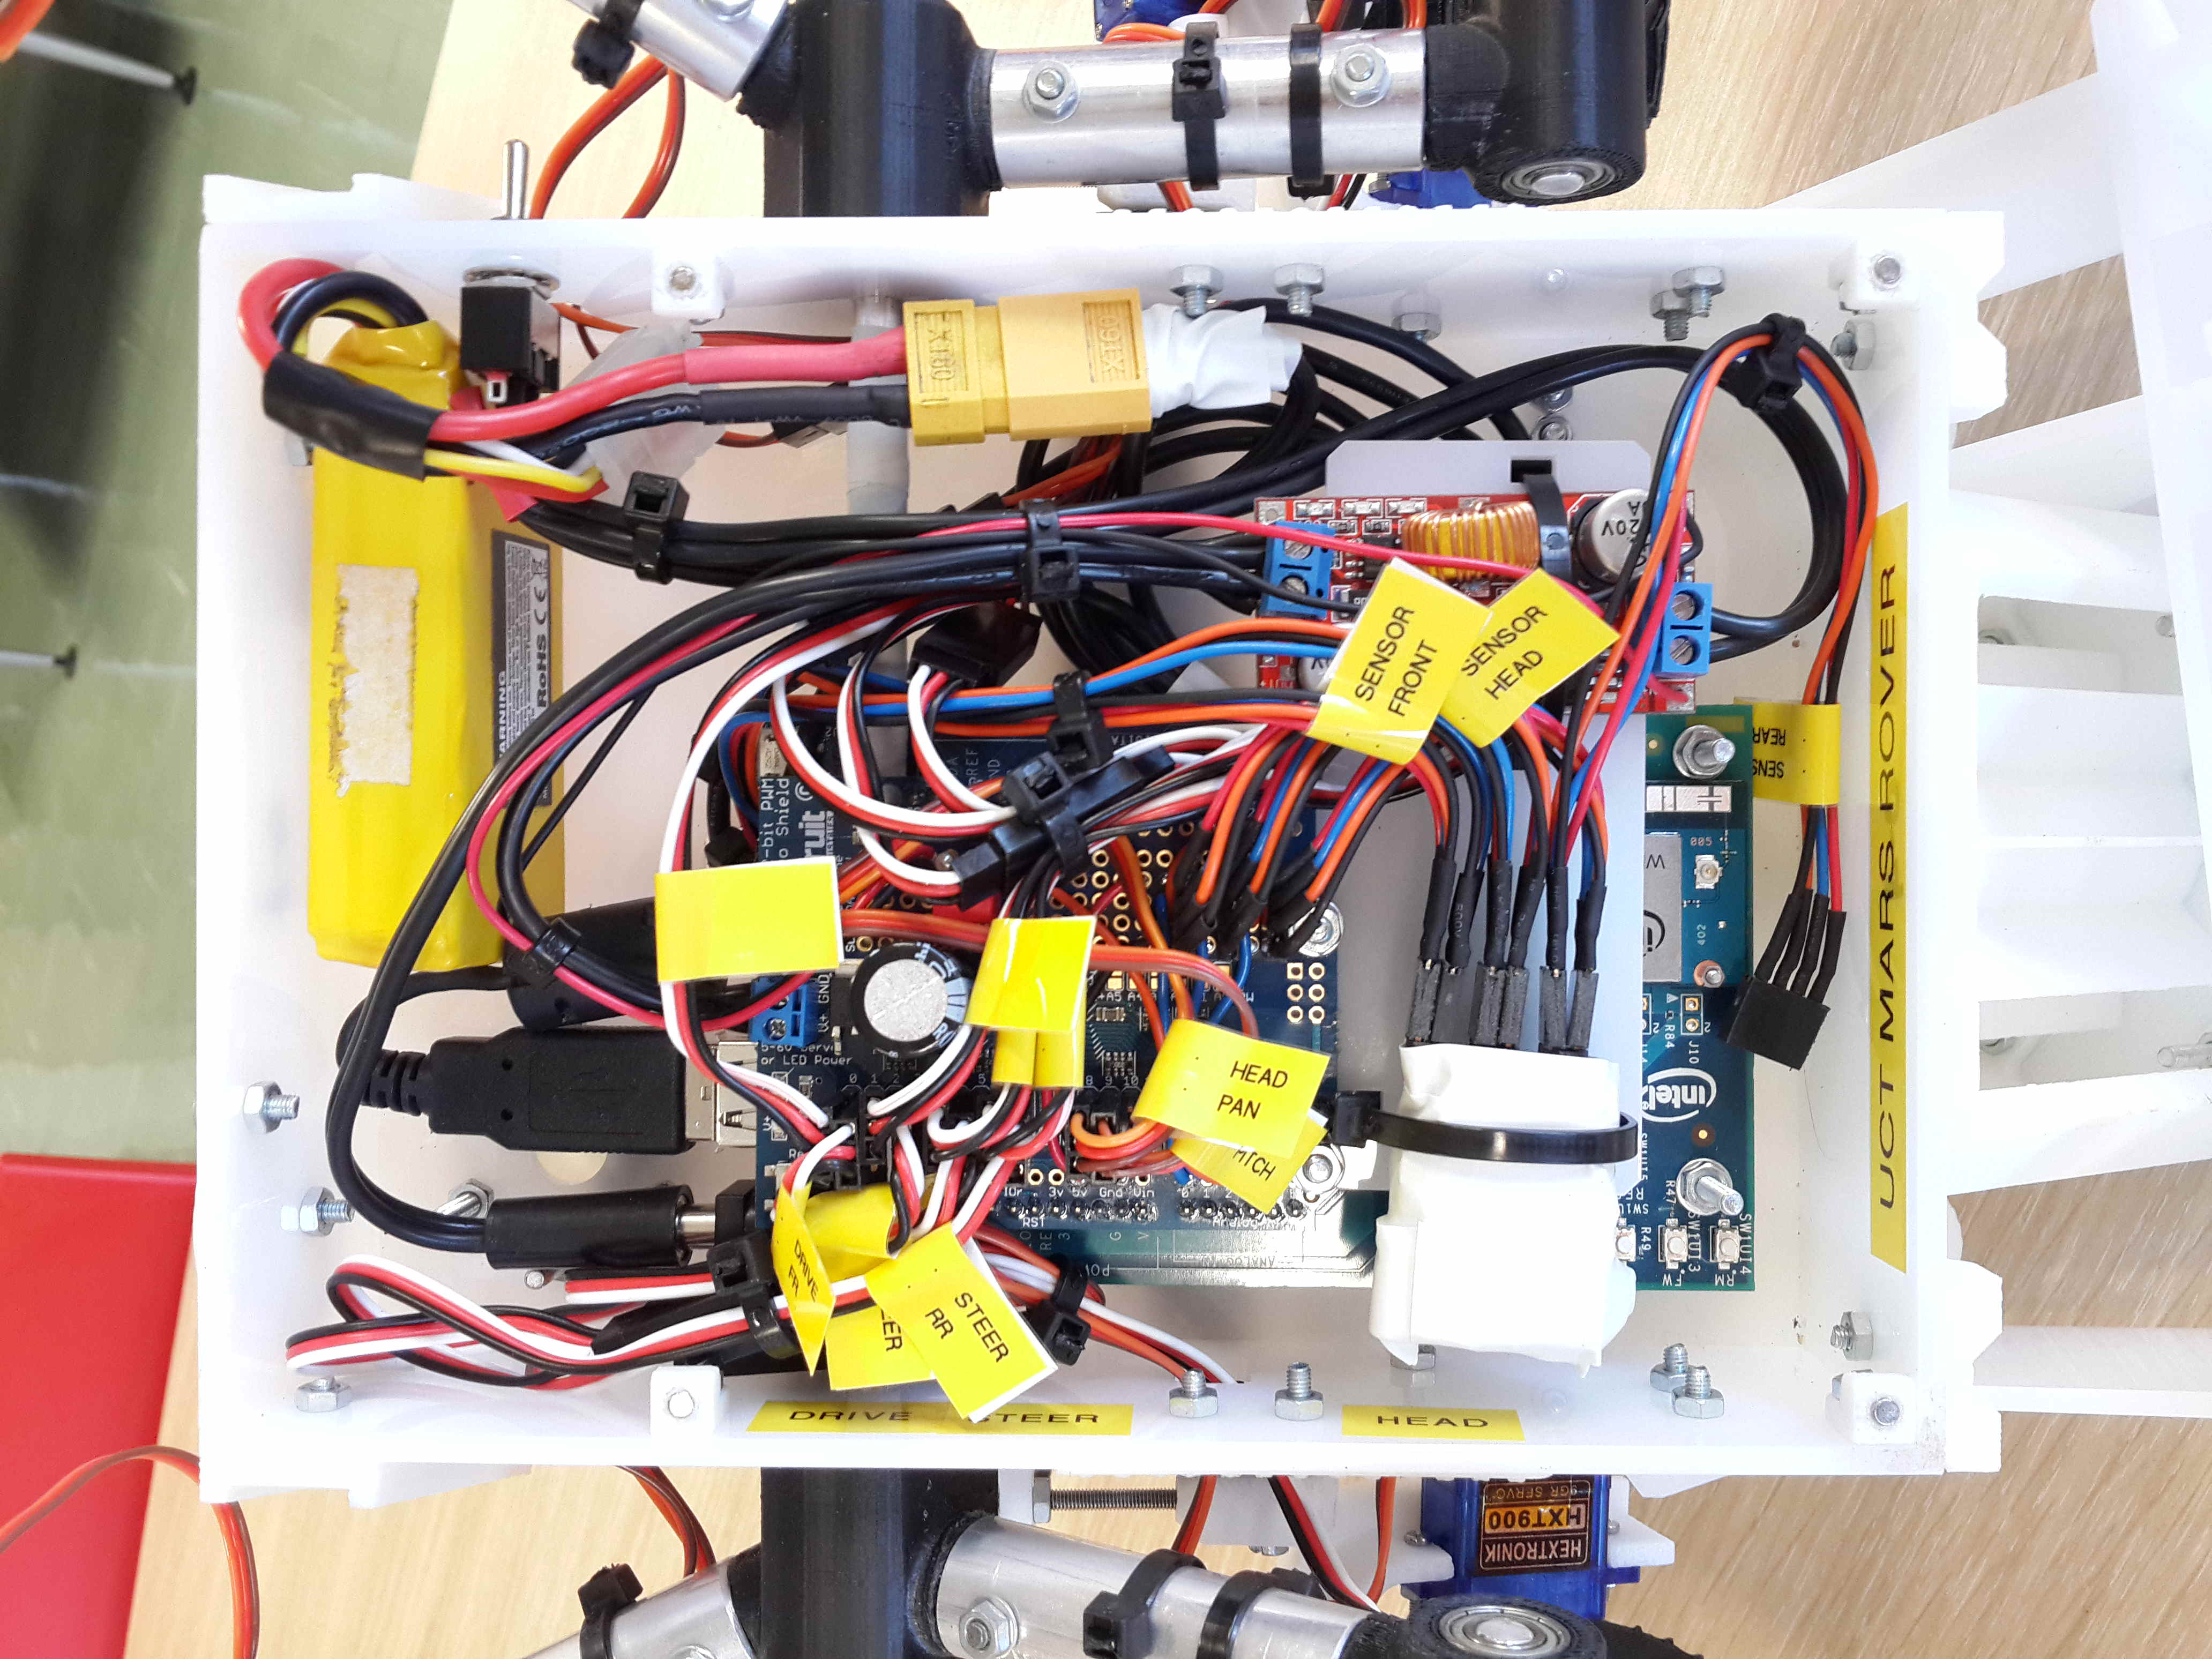
\includegraphics[angle=270, width=0.5\linewidth]{figures/mechBuild-internalElectronics}
        \caption[Image of the fully mounted electronics system including cabling and wiring.]{Image of the fully mounted electronics system including cabling and wiring.}
        \label{fig:mechBuild-internalElectronics}
      \end{figure}
      
      \subheading{Cables and Wiring}
        As seen in Figure~\ref{fig:mechBuild-internalElectronics}, the wiring was neatly packed into the area reserved as in Figure~\ref{fig:mechBuild-internalElectronicsMountingPlan}. Wiring included power cables from the batter to the buck DC to DC converter module and from the module to the Intel Edison board and PWM extension, servo cables, sensor cables and the web camera USB cable. The servo cables, sensor cables and USB cable were fed into the body of the rover through ports included in the acrylic panel design. Servo cables that travelled from the extremities of the suspension system beams were tied to the aluminium tubing with enough slack to cater for the full range of motion of the joints and pivots. The servo and sensor cables were tied and labelled inside the body for easy identification for patching.